\documentclass[tikz,border=2mm]{standalone}
\usepackage{amssymb}
\usepackage{pgfplots}
\usetikzlibrary[arrows.meta]
\usetikzlibrary{positioning, shapes, calc}

\tikzset{set/.style={draw,circle,inner sep=0pt,align=center}}
\tikzset{line/.style = {draw,thick, shorten >=-2pt, shorten <=-2pt}}
\tikzset{tick/.style={draw, minimum width=0pt, minimum height=2pt, inner sep=0pt, label=below:$#1$},tick/.default={}}
\begin{document}
	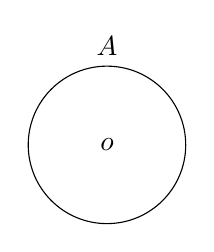
\begin{tikzpicture}[
		node distance=2cm,
		set/.style={draw, circle, minimum size=2cm},
		randomvar/.style={draw, rectangle, minimum size=1.5cm},
		arrow/.style={->, >=stealth, shorten >=2pt, shorten <=2pt}
		]
		% Sample Space Omega
		
		\node[set, label={above:$A$}] (omega) {$o$};
	\end{tikzpicture}
	
	
\end{document}
